\documentclass[11pt]{article}

\usepackage[T1]{fontenc}
\usepackage{lmodern}
\usepackage{amsmath,amssymb,amsthm}
\usepackage{booktabs}
\usepackage{array}
\usepackage{longtable}
\usepackage{graphicx}
\usepackage{tikz-cd}
\usepackage[margin=1in]{geometry}
\usepackage{microtype}
\usepackage[hidelinks]{hyperref}

\theoremstyle{definition}
\newtheorem{definition}{Definition}
\newtheorem{proposition}{Proposition}
\newcommand{\sig}[1]{\left\{#1\right\}}
\newcommand{\impl}{\preccurlyeq_{\mathrm{impl}}}

\title{Exchange Rates for Finite Map Signatures\\
\large A Simplified Thermodynamic Complexity}
\author{Artem Vorozhtsov}
\date{July 2026}

\hypersetup{
  pdftitle={Exchange Rates for Finite Map Signatures},
  pdfauthor={Artem Vorozhtsov}
}

\begin{document}
\maketitle

\begin{abstract}
To a surjection between finite sets we assign the multiset of its fiber
cardinalities.  We compare these signatures by allowing injective
preprocessing and bijective relabelling of the outputs, and define an
asymptotic exchange rate from Cartesian powers.  The rate is expressed by an
infimum of ratios of power sums.  After the substitution
\(\epsilon_i=-\log n_i\), the same formula describes homothetic containment
of Gibbs energy--entropy regions.  The two directed rates do not induce a
transitive comparison: \(\sig{5,3}\), \(\sig{3,1,1}\), and \(\sig{6,1}\)
form a strict cycle.  Algebraically, this is an ordered semiring resource
theory for finite deterministic tasks, related to strong Weihrauch
reducibility and to asymptotic tensor restriction.
\end{abstract}

\section{Signatures and implementation}

Let \(f:X\to Y\) be onto and enumerate its output as
\(Y=\{y_1,\ldots,y_r\}\).  The \emph{fiber} over \(y_i\) is the inverse image
\[
  f^{-1}(y_i)=\{x\in X:f(x)=y_i\},
  \qquad n_i=\left|f^{-1}(y_i)\right|.
\]
Order the fiber sizes decreasingly and define the \emph{signature} of \(f\) by
\[
  \sigma(f)=(n_1,\ldots,n_r),\qquad
  n_1\geq\cdots\geq n_r\geq 1,\qquad r=|Y|.
\]
No other information about the map will be used, and we henceforth use the
same letter for a map and its signature.

\begin{definition}[Implemented by]
Let \(a=(a_1,\ldots,a_r)\) and \(b=(b_1,\ldots,b_s)\) be decreasing
signatures.  We say that \(a\) is \emph{implemented by} \(b\), and write
\(a\impl b\), when \(r\leq s\) and
\[
  a_i\leq b_i\qquad(1\leq i\leq r).
\]
\end{definition}

For maps, this means that there is an injective input relabeling
\(h_{\mathrm{in}}\) and a bijection from the used output fibers to the output
of \(f\) such that
\[
  f=h_{\mathrm{out}}\circ g\circ h_{\mathrm{in}}.
\]
More precisely, put
\[
  X'_g=h_{\mathrm{in}}(X_f),
  \qquad
  Y'_g=g(X'_g).
\]
The two inclusions on the right identify the parts of \(X_g\) and \(Y_g\)
actually used by the implementation, and the following diagram commutes:
\[
\begin{tikzcd}[column sep=large,row sep=large]
  X_f
    \arrow[r,"h_{\mathrm{in}}","\cong"']
    \arrow[d,"f"']
  & X'_g
    \arrow[r,hook]
    \arrow[d,"g|_{X'_g}"]
  & X_g
    \arrow[d,"g"]
  \\
  Y_f
  & Y'_g
    \arrow[l,"h_{\mathrm{out}}"',"\cong"]
    \arrow[r,hook]
  & Y_g .
\end{tikzcd}
\]
Unused fibers of \(g\) may be discarded.  Such an implementation exists
precisely when each fiber of \(f\) injects into its assigned fiber of \(g\),
which is the componentwise condition in Definition~1.

Cartesian product multiplies fiber sizes:
\[
  a\otimes b
  =\operatorname{sort}\{a_i b_j:1\leq i\leq r,\ 1\leq j\leq s\}.
\]
Multiplicity is retained, and \(a^{\otimes k}\) denotes the \(k\)-fold
product.

Disjoint union supplies a second operation:
\[
  f\sqcup g:X_f\sqcup X_g\longrightarrow Y_f\sqcup Y_g
\]
has signature
\[
  a+b=\operatorname{sort}(a_1,\ldots,a_r,b_1,\ldots,b_s).
\]
Both operations respect implementation, and Cartesian product distributes
over this sum:
\[
  a\impl b,\ c\impl d
  \quad\Longrightarrow\quad
  a+c\impl b+d,\quad a\otimes c\impl b\otimes d,
  \qquad
  a\otimes(b+c)=(a\otimes b)+(a\otimes c).
\]
After adjoining the empty signature as zero, signatures form an ordered
commutative semiring with multiplicative unit \(\{1\}\).  Here \(+\) is a
classically labelled alternative and \(\otimes\) is parallel composition.
Only the latter enters the exchange rate.

\begin{definition}[Exchange rate]
For signatures \(f\) and \(g\), set
\[
 k_{\max}^{g\leftarrow f}(n)
 =\max\left\{k\geq0:f^{\otimes k}\impl g^{\otimes n}\right\}.
\]
The exchange rate, with the implementer written first, is
\[
  C(g\mid f)
  =\lim_{n\to\infty}\frac{k_{\max}^{g\leftarrow f}(n)}{n}.
\]
\end{definition}

Tensoring optimal implementations at block lengths \(n\) and \(m\) gives
\[
  k_{\max}(n+m)\geq k_{\max}(n)+k_{\max}(m).
\]
Fekete's lemma now yields
\[
  \lim_{n\to\infty}\frac{k_{\max}(n)}{n}
  =\sup_{n\geq1}\frac{k_{\max}(n)}{n},
\]
with \(+\infty\) allowed.  The limit is the operational definition of
\(C(g\mid f)\).

\section{Related frameworks}

The operations above place the construction among semiring resource theories:
implementation is the free conversion, \(+\) is disjoint choice, and
\(\otimes\) combines independent resources.  General accounts of resource
theories and their ordered algebraic structures are given in
\cite{coecke-fritz-spekkens-2016,fritz-2017}.

The one-shot factorization
\[
  f=h_{\mathrm{out}}\circ g\circ h_{\mathrm{in}}
\]
has the form of strong Weihrauch reduction: one call to \(g\), preceded and
followed by fixed processors \cite{brattka-gherardi-pauly-2021}.  Unlike the
computable processors in Weihrauch theory, ours are injective or bijective on
the sets actually used.  This restriction preserves the fiber capacities.

The asymptotic construction is closer to tensor restriction.  Tensors encode
bilinear tasks, linear maps implement restrictions, and tensor product
combines copies.  Strassen's asymptotic spectrum characterizes large tensor
powers by multiplicative monotones \cite{strassen-1988}.  The relative
exponent
\[
  \omega(t,s)
  =\lim_{n\to\infty}\frac1n
    \min\{m:t^{\otimes m}\text{ restricts to }s^{\otimes n}\}
\]
measures resource cost per target copy; it is used, for example, to quantify
irreversibility in matrix multiplication
\cite{christandl-vrana-zuiddam-2021}.  Its convention is reciprocal to ours
after reversing the conversion.  Here the spectral monotones are the power
sums \(Z_a(\beta)\).  The resulting formula is also analogous to exact
asymptotic majorization, where the rate is a minimum of R\'enyi-entropy ratios
\cite{jensen-2019}.

Channel simulation provides a third comparison: an encoder and decoder use
copies of one channel to reproduce another.  With common-randomness
assistance, the first-order rate for point-to-point discrete memoryless
channels is the ratio of their capacities \cite{cao-et-al-2024}.  Appendix~A
recovers the corresponding logarithmic cardinality ratio when both
processors in the finite-map model are left unrestricted.

\section{Power sums and Gibbs curves}

For a signature \(a=(a_i)\), define its power-sum partition function
\[
  Z_a(\beta)=\sum_i a_i^\beta,\qquad \beta\geq0,
\]
where \(\beta=1/T\) is inverse temperature.  The semiring operations become ordinary addition and
multiplication:
\[
  Z_{a+b}(\beta)=Z_a(\beta)+Z_b(\beta),
  \qquad
  Z_{a\otimes b}(\beta)=Z_a(\beta)Z_b(\beta).
\]
The fibers of the \(k\)-fold Cartesian power \(a^{\otimes k}\) are indexed by
\((i_1,\ldots,i_k)\) and have sizes \(a_{i_1}\cdots a_{i_k}\).  Therefore
\begin{align}
  Z_{a^{\otimes k}}(\beta)
  &=\sum_{i_1,\ldots,i_k}
    (a_{i_1}\cdots a_{i_k})^\beta \notag\\
  &=\left(\sum_i a_i^\beta\right)^k
   =Z_a(\beta)^k,
  \qquad
  \log Z_{a^{\otimes k}}(\beta)=k\log Z_a(\beta).
  \label{eq:tensor-partition}
\end{align}

\begin{proposition}
\label{prop:rate}
Let \(f\) and \(g\) each have at least two fibers and a fiber of size greater
than one.  Then
\begin{equation}
  \label{eq:rate}
  C(g\mid f)
  =\inf_{\beta\in[0,\infty]}
    \frac{\log Z_g(\beta)}{\log Z_f(\beta)},
\end{equation}
where the value at \(\beta=\infty\) is
\[
  \frac{\log\max_j g_j}{\log\max_i f_i}.
\]
\end{proposition}

\begin{proof}[Proof sketch]
If \(f^{\otimes k}\impl g^{\otimes n}\), applying the power sum at every
\(\beta\geq0\) gives
\[
  Z_f(\beta)^k\leq Z_g(\beta)^n,
  \qquad
  \frac{k}{n}\leq
  \frac{\log Z_g(\beta)}{\log Z_f(\beta)}.
\]
The endpoint \(\beta=\infty\) gives the same inequality for the largest
fibers, so the right-hand side of \eqref{eq:rate} is an upper bound.

For the converse, choose a rational \(k/n\) strictly below that infimum.
Sort the logarithms of the fibers in \(f^{\otimes k\ell}\) and
\(g^{\otimes n\ell}\).  The exponential growth rate of the number of entries
above a fixed threshold is the Legendre transform of
\(\log Z_f\), respectively \(\log Z_g\).  The strict power-sum inequalities,
including the two endpoints, therefore give componentwise domination for all
sufficiently large \(\ell\).  Hence
\(f^{\otimes k\ell}\impl g^{\otimes n\ell}\).  Letting \(k/n\) increase to
the infimum proves the reverse inequality.  This is the type-counting
argument used in exact asymptotic majorization; compare
\cite{jensen-2019}.
\end{proof}

Put
\[
  \epsilon_i=-\log a_i,\qquad
  p_i(T)
  =\frac{e^{-\epsilon_i/T}}{\sum_j e^{-\epsilon_j/T}}
  =\frac{a_i^{1/T}}{Z_a(1/T)}.
\]
The corresponding mean energy and entropy are
\[
  E_a(T)=\sum_i p_i(T)\epsilon_i,\qquad
  H_a(T)=-\sum_i p_i(T)\log p_i(T).
\]
They satisfy
\[
  \log Z_a(1/T)=H_a(T)-\frac{E_a(T)}{T}.
\]
Since the Gibbs distribution of a Cartesian power is a product distribution,
\[
 H_{a^{\otimes k}}(T)=kH_a(T),\qquad
 E_{a^{\otimes k}}(T)=kE_a(T),
\]
and therefore
\[
 E_{a^{\otimes k}}(H)=kE_a(H/k),
\]
so Cartesian powers act by homothety in the \((E,H)\)-plane.

Let \(\Gamma_a\) denote the Gibbs curve
\(\{(E_a(T),H_a(T)):0<T<\infty\}\), completed by its endpoint segments, and
let \(\mathcal R_a\) be the closed convex region between this boundary and
the line \(E=0\).  The quantity
\[
  \log Z_a(\beta)=H_a(T)-\beta E_a(T)
\]
is the offset of the supporting line with normal \((-\beta,1)\).  Proposition
\ref{prop:rate} is therefore equivalent to
\[
 C(g\mid f)
 =\sup\{c\geq0:c\,\mathcal R_f\subseteq\mathcal R_g\}.
\]
Equivalently, \(C(g\mid f)^{-1}\Gamma_g\) is the smallest homothetic copy of
\(\Gamma_g\) whose region contains \(\Gamma_f\).

\section{The pair
\texorpdfstring{\(\sig{2,2}\) and \(\sig{3,1}\)}
{{2,2} and {3,1}}}

Let \(g=\sig{2,2}\) and \(f=\sig{3,1}\).  Every fiber of
\(g^{\otimes n}\) has size \(2^n\).  The largest fiber of
\(f^{\otimes k}\) has size \(3^k\), and the remaining rank constraint is
weaker at the optimum.  Hence
\[
  C(\sig{2,2}\mid\sig{3,1})
  =\frac{\log2}{\log3}
  =0.6309297536\ldots.
\]
The reverse direction is limited at a finite temperature:
\begin{align*}
  C(\sig{3,1}\mid\sig{2,2})
  &=\min_{\beta\geq0}
    \frac{\log(3^\beta+1)}{(\beta+1)\log2} \\
  &=0.9653844417\ldots,
  \qquad
  \beta_*=0.4036799030\ldots,\quad
  T_*=\beta_*^{-1}=2.47721027\ldots.
\end{align*}
Figure~\ref{fig:pair} displays both homotheties.  Solid curves are unscaled;
dotted curves are enlarged by the reciprocal directed rate.  Thin endpoint
segments complete the boundaries, and the fills show the regions
\(\mathcal R_a\).  Because the two levels of \(\sig{2,2}\) coincide, its Gibbs
curve reduces to the point \((-\log2,\log2)\).

\begin{figure}[t]
  \centering
  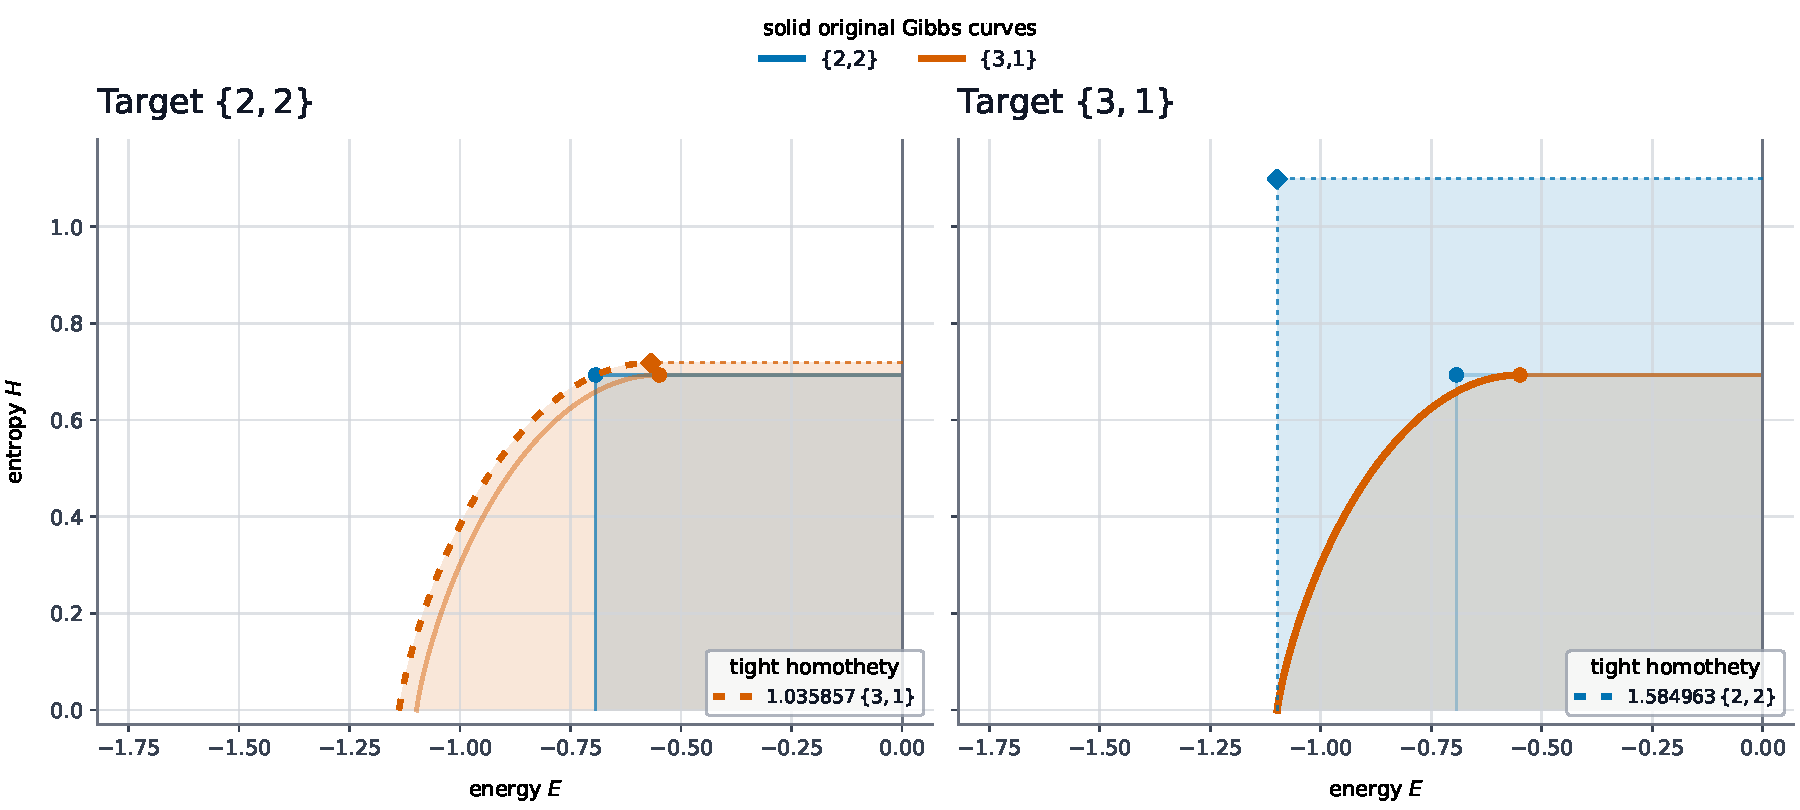
\includegraphics[width=\textwidth]{figures/exchange-homotheties_2-2_3-1.pdf}
  \caption{Exchange rates as planar dilations.  In each panel, one
  energy--entropy region is scaled about the origin until it just contains
  the other.  Thin segments at the \(T=0\) and \(T=\infty\) endpoints close
  the regions; dotted boundaries denote the scaled copy, and translucent
  fills make the containment visible.  The required scale factors are
  \(1/C(\sig{3,1}\mid\sig{2,2})=1.03585676\ldots\) on the left and
  \(1/C(\sig{2,2}\mid\sig{3,1})=\log3/\log2\) on the right.}
  \label{fig:pair}
\end{figure}

\section{A two-sided finite-temperature tangency}

Both directed rates may be attained away from the endpoints.  Consider
\[
  a=\sig{6,5,2,1},
  \qquad
  b=\sig{6,4,3,2}.
\]
The two signatures have equal length and equal largest fiber, so both
endpoint ratios are one:
\[
 \frac{\log Z_a(0)}{\log Z_b(0)}=1,
 \qquad
 \lim_{\beta\to\infty}
 \frac{\log Z_a(\beta)}{\log Z_b(\beta)}
 =\frac{\log6}{\log6}=1.
\]
The interior minima are:
\begin{center}
\begin{tabular}{@{}lrrr@{}}
\toprule
Direction & \(C\) & \(T_*\) & \(\beta_*=1/T_*\) \\
\midrule
\(C(a\mid b)\) &
\(0.9664896992\) & \(1.7970865612\) & \(0.5564562229\) \\
\(C(b\mid a)\) &
\(0.9786567233\) & \(0.2459449336\) & \(4.0659508025\) \\
\bottomrule
\end{tabular}
\end{center}
If
\[
  R(\beta)=\frac{\log Z_g(\beta)}{\log Z_f(\beta)}
\]
has an interior minimum at \(\beta_*\), then \(R'(\beta_*)=0\) and
\(\log Z=H-\beta E\) give
\[
  E_g(T_*)=C(g\mid f)E_f(T_*),
  \qquad
  H_g(T_*)=C(g\mid f)H_f(T_*).
\]
The target curve and the scaled source curve therefore meet at the same
point.  Their slopes also agree, since
\[
  \frac{dH}{dE}=\frac{1}{T_*}=\beta_*,
\]
and this slope is invariant under homothety.  The two contacts in
Figure~\ref{fig:finite-temperature} are genuine tangencies.

\begin{figure}[t]
  \centering
  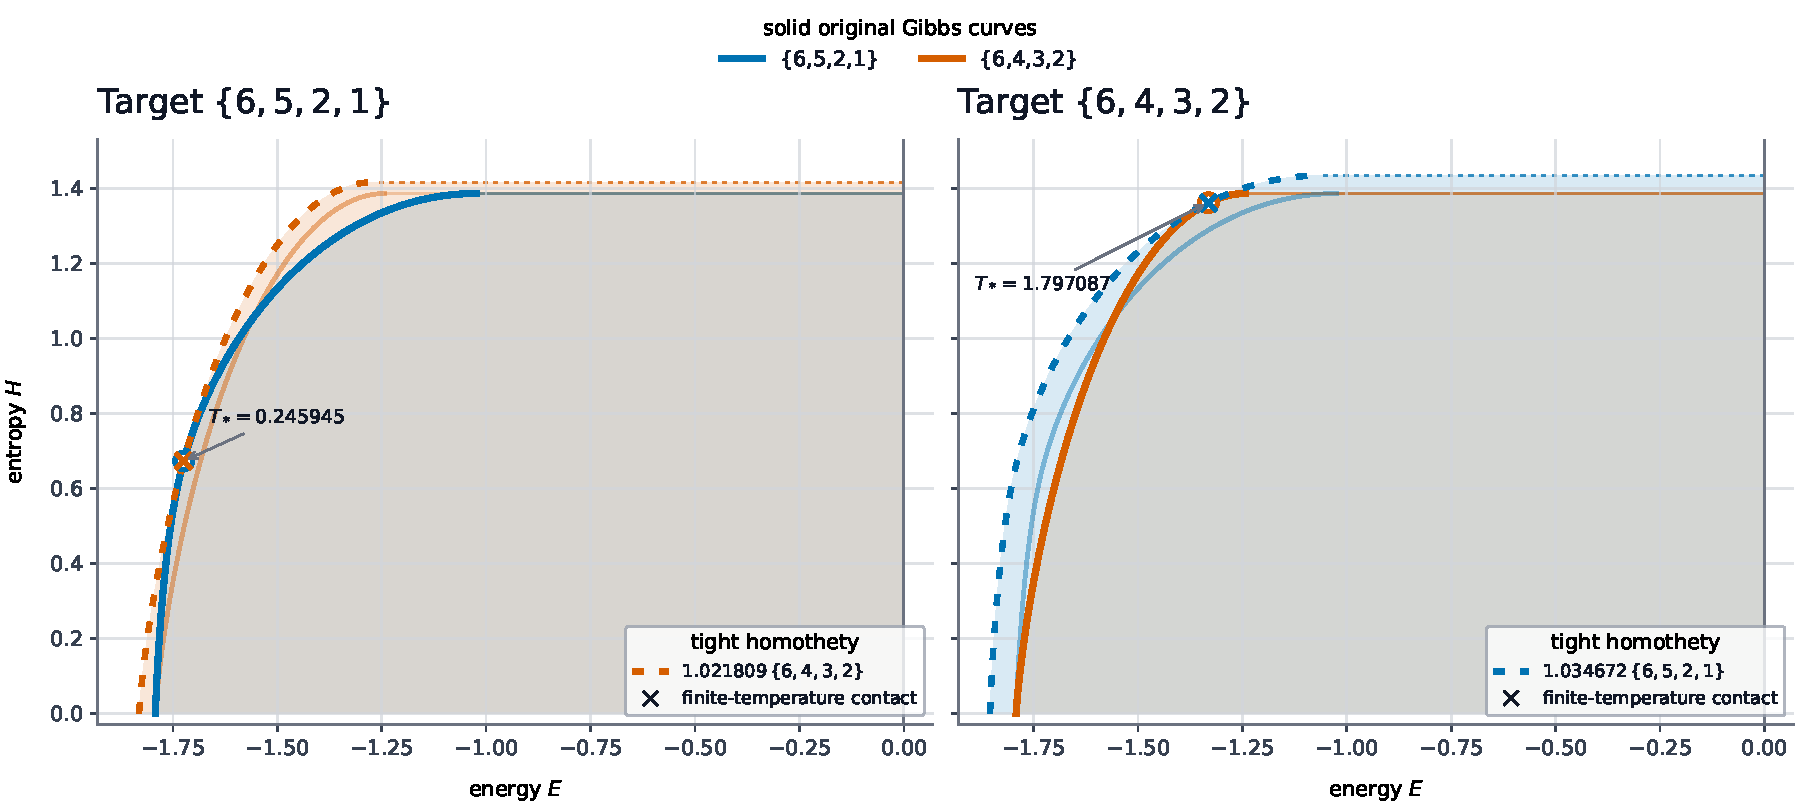
\includegraphics[width=\textwidth]{figures/exchange-homotheties_6-5-2-1_6-4-3-2.pdf}
  \caption{Two-sided finite-temperature tangency.  The left panel scales
  \(b\) by \(1/C(b\mid a)\) to embrace \(a\); the right panel scales \(a\)
  by \(1/C(a\mid b)\) to embrace \(b\).  Crosses mark the interior contact
  points.  Thin dotted horizontal lines close the scaled regions at their
  \(T=\infty\) endpoints; translucent fills extend to \(E=0\).}
  \label{fig:finite-temperature}
\end{figure}

\section{A cyclic strict comparison}
\label{sec:strict-cycle}

\begin{definition}
For signatures \(a,b\), define
\[
  a\prec b
  \quad\Longleftrightarrow\quad
  C(a\mid b)<C(b\mid a).
\]
\end{definition}

In this terminology, \(b\) is more complex than \(a\) when conversion from
\(b\) to \(a\) is more efficient than conversion in the opposite direction.
The relation is not transitive.

Set
\[
  f_1=\sig{5,3},\qquad
  f_2=\sig{3,1,1},\qquad
  f_3=\sig{6,1}.
\]
Equation \eqref{eq:rate} gives the comparisons in
Table~\ref{tab:cycle}.

\begin{table}[ht]
  \centering
  \caption{Directed rates producing a strict cycle.}
  \label{tab:cycle}
  \begin{tabular}{@{}cccc@{}}
    \toprule
    Pair & Forward rate & Reverse rate & Conclusion \\
    \midrule
    \(f_1,f_2\) & \(C(f_1\mid f_2)=0.630929754\)
                & \(C(f_2\mid f_1)=0.670211928\) & \(f_1\prec f_2\) \\
    \(f_2,f_3\) & \(C(f_2\mid f_3)=0.613147193\)
                & \(C(f_3\mid f_2)=0.630929754\) & \(f_2\prec f_3\) \\
    \(f_3,f_1\) & \(C(f_3\mid f_1)=0.897931851\)
                & \(C(f_1\mid f_3)=0.898244402\) & \(f_3\prec f_1\) \\
    \bottomrule
  \end{tabular}
\end{table}

The three rows give
\[
  f_1\prec f_2,\qquad f_2\prec f_3,\qquad f_3\prec f_1.
\]
Hence \(\prec\) is not a strict order.  Figure~\ref{fig:cycle} shows the three
comparisons geometrically.  In the panel with target \(f_i\), the dotted curve
for \(f_j\) is \(C(f_j\mid f_i)^{-1}\Gamma_{f_j}\).

\begin{figure}[t]
  \centering
  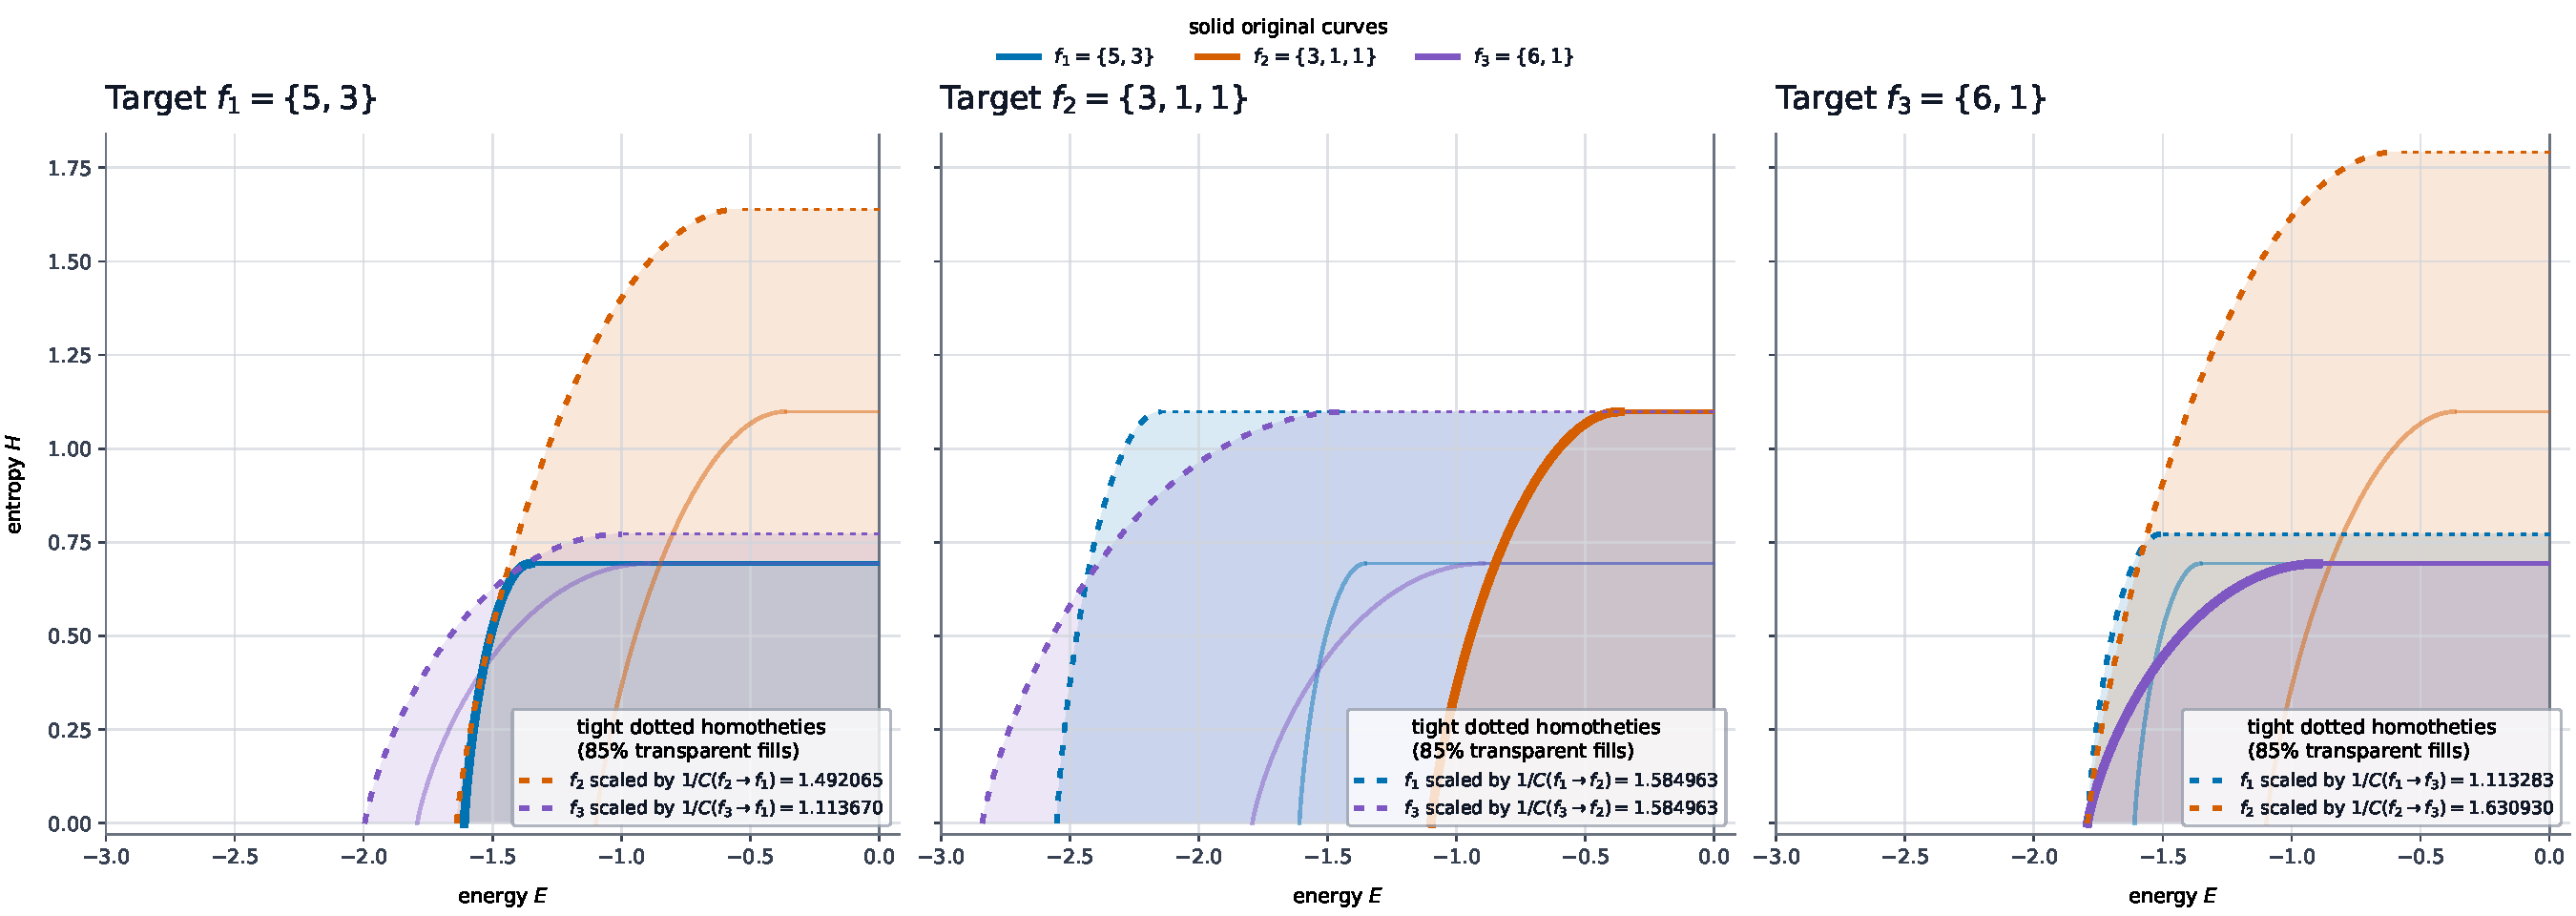
\includegraphics[width=\textwidth]{figures/exchange-homotheties_cycle-5-3_3-1-1_6-1.pdf}
  \caption{The cyclic example.  Solid and dotted boundaries are original and
  scaled, respectively.  Horizontal \(T=\infty\) closures and
  85\%-transparent fills extending to \(E=0\) display target containment.}
  \label{fig:cycle}
\end{figure}

\section{A thermodynamic analogy and its limits}

Associate signatures \(A=(a_i)\) and \(B=(b_j)\) with two idealized particle
species whose internal energy levels are
\[
  \epsilon_i^A=-\log a_i,
  \qquad
  \epsilon_j^B=-\log b_j.
\]
Then \(A^{\otimes k}\) and \(B^{\otimes n}\) represent \(k\) noninteracting
particles of type \(A\) and \(n\) noninteracting particles of type \(B\),
respectively.  If their scaled Gibbs curves are tangent at interior points,
\[
  \frac{dH_A}{dE_A}
  =
  \frac{dH_B}{dE_B}
  =
  \frac{1}{T}.
\]
The tangent Gibbs states therefore have the same temperature.

This identification is kinematic, not dynamical: \(\impl\) records an allowed
combinatorial conversion, not a reaction mechanism.  For the formal
stoichiometry
\[
  kA\rightleftharpoons nB
\]
write \(r=k/n\).  In the asymptotic closure,
\begin{align}
  B^{\otimes n}\longrightarrow A^{\otimes k}
  &\quad\Longleftrightarrow\quad r\leq C(B\mid A),
  \label{eq:B-to-A}\\
  A^{\otimes k}\longrightarrow B^{\otimes n}
  &\quad\Longleftrightarrow\quad
  r\geq \frac{1}{C(A\mid B)}.
  \label{eq:A-to-B}
\end{align}
Strict inequalities guarantee the corresponding direction for sufficiently
large block sizes; an exact boundary ratio need not be attained at finite
size.  Since
\[
  C(A\mid B)C(B\mid A)\leq1,
\]
the thresholds leave the interval
\[
  C(B\mid A)\leq r\leq\frac{1}{C(A\mid B)}.
\]
For ratios in its interior, neither direction need realize the prescribed
stoichiometry.  Coincident endpoints mean asymptotic reversibility; otherwise
the interval measures irreversibility.

Physical equilibrium requires more.  At fixed temperature and pressure the
reaction affinity must vanish:
\[
  \mathcal A=k\mu_A-n\mu_B=0,
\]
where \(\mu_A\) and \(\mu_B\) are chemical potentials.  Neither chemical
potentials nor reaction kinetics occur in our definition.  Equations
\eqref{eq:B-to-A}--\eqref{eq:A-to-B} therefore describe allowed conversions,
not spontaneous reaction directions.

The strict cycle admits a formal comparison with a driven reaction network.
For \(a\overset{\mathrm{s}}{\longrightarrow}b\), set
\[
  \alpha(a\to b)
  =\log\frac{C(a\mid b)}{C(b\mid a)}>0.
\]
For the cycle of Section~\ref{sec:strict-cycle},
\[
  f_1\overset{\mathrm{s}}{\longrightarrow}f_3
  \overset{\mathrm{s}}{\longrightarrow}f_2
  \overset{\mathrm{s}}{\longrightarrow}f_1,
\]
the sum around the cycle is
\[
\begin{split}
  \mathcal A_{\mathrm{cyc}}
  ={}&\alpha(f_1\to f_3)+\alpha(f_3\to f_2)+\alpha(f_2\to f_1)\\
  ={}&
  \log\frac{0.898244402}{0.897931851}
  +\log\frac{0.630929754}{0.613147193}
  +\log\frac{0.670211928}{0.630929754}\\
  ={}&0.089337,
  \qquad e^{\mathcal A_{\mathrm{cyc}}}=1.09345.
\end{split}
\]
If \(\alpha\) is read as a logarithmic forward--reverse bias, the orientation
matches the reaction network
\[
  A\rightleftharpoons B,\qquad
  B\rightleftharpoons C,\qquad
  C\rightleftharpoons A.
\]

It cannot represent circulation in a closed equilibrium gas.  Reaction
affinity is the negative derivative of Gibbs energy with respect to reaction
extent \cite{iupac-affinity}; detailed balance forces the affinity around a
closed cycle to vanish.  Nonzero cycle affinity instead belongs to an open
system maintained by reservoirs.  Such networks are studied in
\cite{polettini-esposito-2014,rao-esposito-2016}; a stochastic
three-species example appears in \cite{schmiedl-seifert-2007}.

The analogy stops at this structural resemblance.  The rates \(C(a\mid b)\)
are not kinetic constants, and the three minima may occur at different
temperatures.  Without kinetics, conservation laws, or external work
accounting, the strict cycle predicts neither a current nor an oscillation.

A fixed reaction energy can be included as an offset.  For
\[
  kA\rightleftharpoons nB+q
\]
shift every level of \(B\) by \(q/n\):
\[
  \widetilde\epsilon_{B,j}=\epsilon_{B,j}+\frac qn.
\]
Then
\[
  \widetilde E_B(H)=E_B(H)+\frac qn,\qquad
  \widetilde Z_B(1/T)=e^{-q/(nT)}Z_B(1/T),
\]
while \(H_B(T)\) and \(dH_B/dE=1/T\) are unchanged.  The \(n\)-particle
region is therefore translated horizontally by \(q\).  This accounts for a
fixed offset carried by a work-storage degree of freedom; heat transfer to a
bath cannot be represented by a horizontal shift alone.

The model omits interactions, quantum statistics, translational and volume
degrees of freedom, mixing entropy, conservation laws, kinetics, activation
barriers, and reservoirs.  Its energies are dimensionless (\(k_B=1\)), and
relative offsets between particle types must be fixed whenever particle
number can change.  These omissions delimit the analogy.

The supporting function
\[
  \Psi_A(T)=\log Z_A(1/T)=-\frac{F_A(T)}{T}
\]
is the Massieu potential.  Proposition~\ref{prop:rate} becomes
\[
  C(A\mid B)=\inf_{T>0}\frac{\Psi_A(T)}{\Psi_B(T)}
\]
and asks for the largest \(c\) such that
\(\Psi_A(T)\geq c\Psi_B(T)\) for every \(T\).  An interior minimizer is the
bottleneck temperature.  Sparaciari, Oppenheim, and Fritz study a related
resource theory without a fixed background temperature, in which asymptotic
rates are read from an energy--entropy diagram
\cite{sparaciari-oppenheim-fritz-2017}.  Our comparison uses the whole Gibbs
boundary rather than a single prescribed heat bath.

\begin{figure}[t]
  \centering
  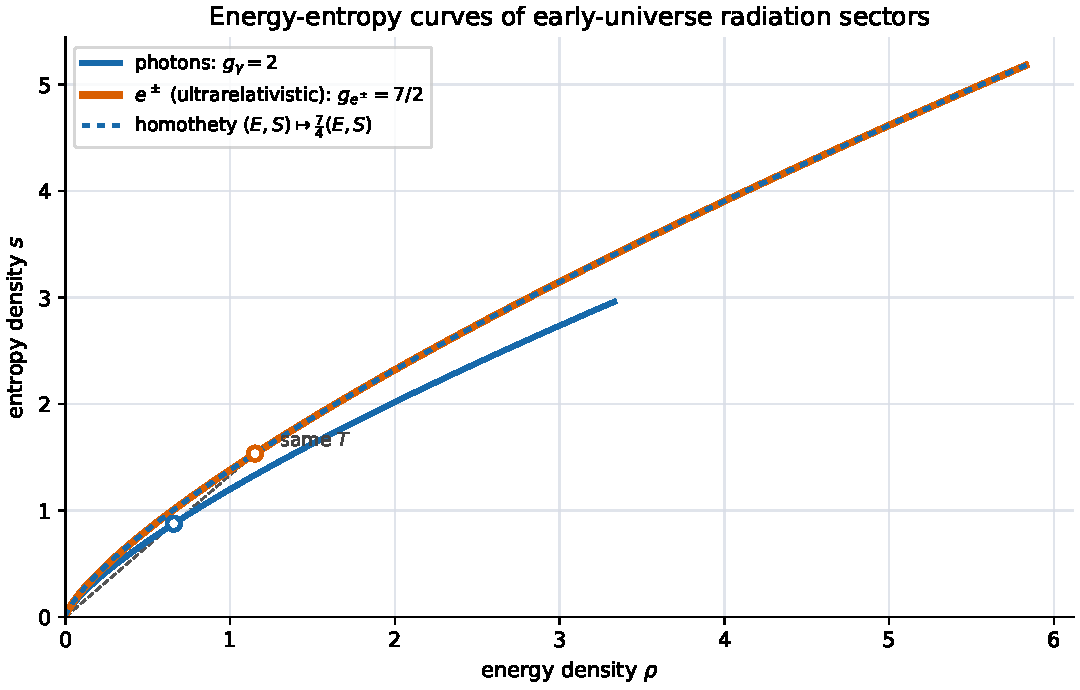
\includegraphics[width=0.78\textwidth]{figures/relativistic-radiation-energy-entropy.pdf}
  \caption{Exact homothety in the ultrarelativistic limit.  At fixed
  temperature, the electron--positron sector has \(7/4\) times the energy and
  entropy densities of the photon sector; the rescaled photon curve therefore
  coincides with it.}
  \label{fig:radiation-sectors}
\end{figure}

An exact physical homothety occurs for ultrarelativistic equilibrium sectors.
If \(g_X\) is the effective number of internal degrees of freedom, then in
natural units and at fixed volume
\[
  E_X(T)=\frac{\pi^2}{30}g_XVT^4,\qquad
  H_X(T)=\frac{2\pi^2}{45}g_XVT^3.
\]
Therefore
\[
  E_A(T)=\frac{g_A}{g_B}E_B(T),\qquad
  H_A(T)=\frac{g_A}{g_B}H_B(T)
\]
at every temperature, so the two boundaries are homothetic with factor
\(g_A/g_B\).  For photons \(g_\gamma=2\); for an ultrarelativistic
electron--positron sector \(g_{e^\pm}=(7/8)\times4=7/2\).  The factor is
therefore \(7/4\), as in Figure~\ref{fig:radiation-sectors}.  In the early
universe, \(e^-+e^+\rightleftharpoons2\gamma\) maintained equilibrium until
the temperature fell below the electron mass and annihilation transferred
entropy to the photon bath \cite{thomas-et-al-2020}.

For general Gibbs systems, homothetic containment is at present a proposed
complexity measure.  Infinite spectra and an operational conversion model
require separate treatment.

\section{Conclusion}

A fiber signature is a coarse invariant of a finite map, but Cartesian powers
already give it a nontrivial asymptotic conversion theory.  The operational
rate, the power-sum formula, and containment of Gibbs regions are equivalent
descriptions of that theory.  The directed rates cannot be compressed into a
global ranking, as the explicit three-cycle shows.  Extending Gibbs-region
containment beyond finite signatures remains plausible, but it requires an
operational model distinct from chemical reaction dynamics.

\begin{thebibliography}{99}
\raggedright

\bibitem{coecke-fritz-spekkens-2016}
B.~Coecke, T.~Fritz, and R.~W.~Spekkens,
``A mathematical theory of resources,''
\emph{Information and Computation} \textbf{250}, 59--86 (2016).
\href{https://doi.org/10.1016/j.ic.2016.02.008}
{doi:10.1016/j.ic.2016.02.008}.

\bibitem{fritz-2017}
T.~Fritz,
``Resource convertibility and ordered commutative monoids,''
\emph{Math. Struct. Comput. Sci.} \textbf{27}, 850--938 (2017).
\href{https://doi.org/10.1017/S0960129515000444}
{doi:10.1017/S0960129515000444}.

\bibitem{brattka-gherardi-pauly-2021}
V.~Brattka, G.~Gherardi, and A.~Pauly,
``Weihrauch complexity in computable analysis,''
in \emph{Handbook of Computability and Complexity in Analysis},
pp.~367--417 (Springer, Cham, 2021).
\href{https://doi.org/10.1007/978-3-030-59234-9_11}
{doi:10.1007/978-3-030-59234-9\_11}.

\bibitem{strassen-1988}
V.~Strassen,
``The asymptotic spectrum of tensors,''
\emph{J. Reine Angew. Math.} \textbf{384}, 102--152 (1988).
\href{https://doi.org/10.1515/crll.1988.384.102}
{doi:10.1515/crll.1988.384.102}.

\bibitem{christandl-vrana-zuiddam-2021}
M.~Christandl, P.~Vrana, and J.~Zuiddam,
``Barriers for fast matrix multiplication from irreversibility,''
\emph{Theory Comput.} \textbf{17}(2), 1--32 (2021).
\href{https://doi.org/10.4086/toc.2021.v017a002}
{doi:10.4086/toc.2021.v017a002}.

\bibitem{jensen-2019}
A.~Kj{\ae}rulff Jensen,
``Asymptotic majorization of finite probability distributions,''
\emph{IEEE Trans. Inf. Theory} \textbf{65}, 8131--8139 (2019).
\href{https://doi.org/10.1109/TIT.2019.2922627}
{doi:10.1109/TIT.2019.2922627}.

\bibitem{cao-et-al-2024}
M.~X.~Cao, N.~Ramakrishnan, M.~Berta, and M.~Tomamichel,
``Channel simulation: finite blocklengths and broadcast channels,''
\emph{IEEE Trans. Inf. Theory} \textbf{70}, 6780--6808 (2024).
\href{https://doi.org/10.1109/TIT.2024.3445998}
{doi:10.1109/TIT.2024.3445998};
\href{https://arxiv.org/abs/2212.11666}{arXiv:2212.11666}.

\bibitem{iupac-affinity}
International Union of Pure and Applied Chemistry,
``Affinity of reaction,''
\emph{Compendium of Chemical Terminology (the Gold Book)}, 5th ed.,
online version 5.0.0 (2025).
\href{https://doi.org/10.1351/goldbook.A00178}
{doi:10.1351/goldbook.A00178}.

\bibitem{polettini-esposito-2014}
M.~Polettini and M.~Esposito,
``Irreversible thermodynamics of open chemical networks I:
emergent cycles and broken conservation laws,''
\emph{J. Chem. Phys.} \textbf{141}, 024117 (2014).
\href{https://doi.org/10.1063/1.4886396}{doi:10.1063/1.4886396}.

\bibitem{rao-esposito-2016}
R.~Rao and M.~Esposito,
``Nonequilibrium thermodynamics of chemical reaction networks:
wisdom from stochastic thermodynamics,''
\emph{Phys. Rev. X} \textbf{6}, 041064 (2016).
\href{https://doi.org/10.1103/PhysRevX.6.041064}
{doi:10.1103/PhysRevX.6.041064}.

\bibitem{schmiedl-seifert-2007}
T.~Schmiedl and U.~Seifert,
``Stochastic thermodynamics of chemical reaction networks,''
\emph{J. Chem. Phys.} \textbf{126}, 044101 (2007).
\href{https://doi.org/10.1063/1.2428297}{doi:10.1063/1.2428297}.

\bibitem{sparaciari-oppenheim-fritz-2017}
C.~Sparaciari, J.~Oppenheim, and T.~Fritz,
``A resource theory for work and heat,''
\emph{Phys. Rev. A} \textbf{96}, 052112 (2017).
\href{https://doi.org/10.1103/PhysRevA.96.052112}
{doi:10.1103/PhysRevA.96.052112}.

\bibitem{thomas-et-al-2020}
L.~C.~Thomas, T.~Dezen, E.~B.~Grohs, and C.~T.~Kishimoto,
``Electron-positron annihilation freeze-out in the early universe,''
\emph{Phys. Rev. D} \textbf{101}, 063507 (2020).
\href{https://doi.org/10.1103/PhysRevD.101.063507}
{doi:10.1103/PhysRevD.101.063507}.

\end{thebibliography}

\appendix
\section{Unrestricted input and output maps}

Suppose that the maps \(h_{\mathrm{in}}\) and \(h_{\mathrm{out}}\) in the
definition of implementation are unrestricted.  Then \(b\) is implementable
by \(a\) if and only if
\[
  |Y_b|\leq |Y_a|.
\]
An arbitrary \(h_{\mathrm{in}}\) may collapse each fiber of \(b\) onto one
chosen input of \(a\), so only the number of available output fibers remains.
A deterministic \(h_{\mathrm{out}}\) cannot increase that number.

For Cartesian powers the condition is therefore
\[
  |Y_b|^k\leq |Y_a|^n,
  \qquad
  k_{\max}(n)
  =\left\lfloor
    n\frac{\log|Y_a|}{\log|Y_b|}
   \right\rfloor.
\]
Hence, for \(|Y_a|,|Y_b|>1\),
\[
  \boxed{\displaystyle
  C(a\mid b)=\frac{\log|Y_a|}{\log|Y_b|}}.
\]
The same ratio appears in assisted point-to-point channel interconversion
\cite{cao-et-al-2024}: a surjective deterministic channel with output set
\(Y\) has capacity \(\log|Y|\).  Unrestricted processors retain only this
capacity; the processors of Definition~1 also retain the individual fiber
sizes.

\(C(a\mid b)C(b\mid a)=1\), so the comparison from
Definition~3 reduces to
\[
  a\prec b
  \quad\Longleftrightarrow\quad
  |Y_a|<|Y_b|.
\]
This is a total preorder, and quotienting by equal output cardinality gives a
linear order.  In partition-function language only
\(Z_a(0)=|Y_a|\) remains.  If \(|Y_b|=1\), then
\(C(a\mid b)=+\infty\); if \(|Y_a|=1<|Y_b|\), then \(C(a\mid b)=0\).

\section{The first 69 non-special signatures}

We omit the exceptional infinite families \(\sig{N}\) and
\(\sig{1,\ldots,1}\).  To enumerate every other signature without imposing a
fixed length or entry bound, put
\[
  \mathcal S_B
  =\{a:|a|\geq2,\ a_1>1,\ a_1+2|a|\leq B\}.
\]
Every non-special signature eventually belongs to \(\mathcal S_B\).  For each
\(B\), the strongly connected components of the strict comparison graph are
contracted and topologically ordered by the deterministic rule implemented in
the analysis code.  At the stated screening precision, the first 69 entries
agree for \(B=18,19,20\).  Table~\ref{tab:first-69-signatures} records this
stable prefix; its rates were recomputed from the high-accuracy cache.

Because \(\prec\) is not transitive, this list is not a linear extension of
all pairwise comparisons.  A row for \(x\) in
Table~\ref{tab:signature-order-exceptions} records each earlier \(a\) for
which
\[
  C(x\mid a)<C(a\mid x)
\]
despite the displayed order \(a<x\).

% Generated by analysis/appendix_b_signatures.py.
\begingroup
\footnotesize
\begin{longtable}{@{}r l@{\qquad}r l@{\qquad}r l@{}}
  \caption{The first 99 non-special signatures in the deterministic
  condensation-DAG order.}
  \label{tab:first-99-signatures}\\
    \toprule
    \(n\) & signature & \(n\) & signature & \(n\) & signature \\
    \midrule
    1 & \(\sig{2,1}\) & 34 & \(\sig{7,7}\) & 67 & \(\sig{4,4,4}\) \\
    2 & \(\sig{2,2}\) & 35 & \(\sig{8,1}\) & 68 & \(\sig{5,1,1}\) \\
    3 & \(\sig{3,1}\) & 36 & \(\sig{8,2}\) & 69 & \(\sig{5,2,1}\) \\
    4 & \(\sig{2,1,1}\) & 37 & \(\sig{8,3}\) & 70 & \(\sig{5,2,2}\) \\
    5 & \(\sig{3,2}\) & 38 & \(\sig{8,4}\) & 71 & \(\sig{5,3,1}\) \\
    6 & \(\sig{2,2,1}\) & 39 & \(\sig{8,5}\) & 72 & \(\sig{5,3,2}\) \\
    7 & \(\sig{3,3}\) & 40 & \(\sig{8,6}\) & 73 & \(\sig{3,3,3,3}\) \\
    8 & \(\sig{2,1,1,1}\) & 41 & \(\sig{8,7}\) & 74 & \(\sig{4,1,1,1}\) \\
    9 & \(\sig{2,2,2}\) & 42 & \(\sig{3,1,1}\) & 75 & \(\sig{5,4,1}\) \\
    10 & \(\sig{4,1}\) & 43 & \(\sig{3,2,1}\) & 76 & \(\sig{5,3,3}\) \\
    11 & \(\sig{2,2,1,1}\) & 44 & \(\sig{3,2,2}\) & 77 & \(\sig{5,4,2}\) \\
    12 & \(\sig{4,2}\) & 45 & \(\sig{3,3,1}\) & 78 & \(\sig{4,2,1,1}\) \\
    13 & \(\sig{2,2,2,1}\) & 46 & \(\sig{3,3,2}\) & 79 & \(\sig{5,5,1}\) \\
    14 & \(\sig{4,3}\) & 47 & \(\sig{3,3,3}\) & 80 & \(\sig{5,4,3}\) \\
    15 & \(\sig{2,2,2,2}\) & 48 & \(\sig{4,1,1}\) & 81 & \(\sig{4,2,2,1}\) \\
    16 & \(\sig{5,1}\) & 49 & \(\sig{3,1,1,1}\) & 82 & \(\sig{5,5,2}\) \\
    17 & \(\sig{4,4}\) & 50 & \(\sig{4,2,1}\) & 83 & \(\sig{5,4,4}\) \\
    18 & \(\sig{5,2}\) & 51 & \(\sig{4,2,2}\) & 84 & \(\sig{5,5,3}\) \\
    19 & \(\sig{5,3}\) & 52 & \(\sig{8,8}\) & 85 & \(\sig{4,3,1,1}\) \\
    20 & \(\sig{5,4}\) & 53 & \(\sig{3,2,1,1}\) & 86 & \(\sig{4,2,2,2}\) \\
    21 & \(\sig{5,5}\) & 54 & \(\sig{3,2,2,1}\) & 87 & \(\sig{5,5,4}\) \\
    22 & \(\sig{6,1}\) & 55 & \(\sig{3,2,2,2}\) & 88 & \(\sig{4,3,2,1}\) \\
    23 & \(\sig{6,2}\) & 56 & \(\sig{4,3,1}\) & 89 & \(\sig{4,3,2,2}\) \\
    24 & \(\sig{6,3}\) & 57 & \(\sig{3,3,1,1}\) & 90 & \(\sig{5,5,5}\) \\
    25 & \(\sig{6,4}\) & 58 & \(\sig{4,3,2}\) & 91 & \(\sig{4,3,3,1}\) \\
    26 & \(\sig{6,5}\) & 59 & \(\sig{3,3,2,1}\) & 92 & \(\sig{4,4,1,1}\) \\
    27 & \(\sig{6,6}\) & 60 & \(\sig{4,4,1}\) & 93 & \(\sig{4,3,3,2}\) \\
    28 & \(\sig{7,1}\) & 61 & \(\sig{3,3,2,2}\) & 94 & \(\sig{4,4,2,1}\) \\
    29 & \(\sig{7,2}\) & 62 & \(\sig{3,3,3,1}\) & 95 & \(\sig{4,3,3,3}\) \\
    30 & \(\sig{7,3}\) & 63 & \(\sig{3,3,3,2}\) & 96 & \(\sig{4,4,2,2}\) \\
    31 & \(\sig{7,4}\) & 64 & \(\sig{4,3,3}\) & 97 & \(\sig{4,4,3,1}\) \\
    32 & \(\sig{7,5}\) & 65 & \(\sig{4,4,2}\) & 98 & \(\sig{4,4,3,2}\) \\
    33 & \(\sig{7,6}\) & 66 & \(\sig{4,4,3}\) & 99 & \(\sig{4,4,4,1}\) \\
    \bottomrule
\end{longtable}
\endgroup

\begin{longtable}{@{}r l >{\raggedright\arraybackslash}p{0.67\textwidth}@{}}
  \caption{Backward comparisons that obstruct a linear order.}
  \label{tab:signature-order-exceptions}\\
  \toprule
  \(n\) & \(x\) & exceptions with previous \(n_a\) values \\
  \midrule
  \endfirsthead
  \multicolumn{3}{@{}l}{\small\itshape Table \thetable\ continued from the previous page}\\
  \toprule
  \(n\) & \(x\) & exceptions with previous \(n_a\) values \\
  \midrule
  \endhead
  \midrule
  \multicolumn{3}{r@{}}{\small continued on the next page}\\
  \endfoot
  \bottomrule
  \endlastfoot
  22 & \(\sig{6,1}\) & \(n_a\in\{19\}\):\newline \(\quad C(x\!\mid\!a)=0.897932,\ C(a\!\mid\!x)=0.898244\)\newline \(n_a\in\{20\}\):\newline \(\quad C(x\!\mid\!a)=0.857550,\ C(a\!\mid\!x)=0.898244\)\newline \(n_a\in\{21\}\):\newline \(\quad C(x\!\mid\!a)=0.825066,\ C(a\!\mid\!x)=0.898244\) \\
  \cmidrule(lr){1-3}
  28 & \(\sig{7,1}\) & \(n_a\in\{24\}\):\newline \(\quad C(x\!\mid\!a)=0.902627,\ C(a\!\mid\!x)=0.920782\)\newline \(n_a\in\{25\}\):\newline \(\quad C(x\!\mid\!a)=0.866396,\ C(a\!\mid\!x)=0.920782\)\newline \(n_a\in\{26\}\):\newline \(\quad C(x\!\mid\!a)=0.837432,\ C(a\!\mid\!x)=0.920782\)\newline \(n_a\in\{27\}\):\newline \(\quad C(x\!\mid\!a)=0.813202,\ C(a\!\mid\!x)=0.920782\) \\
  \cmidrule(lr){1-3}
  29 & \(\sig{7,2}\) & \(n_a\in\{26\}\):\newline \(\quad C(x\!\mid\!a)=0.906054,\ C(a\!\mid\!x)=0.920782\)\newline \(n_a\in\{27\}\):\newline \(\quad C(x\!\mid\!a)=0.878094,\ C(a\!\mid\!x)=0.920782\) \\
  \cmidrule(lr){1-3}
  35 & \(\sig{8,1}\) & \(n_a\in\{27\}\):\newline \(\quad C(x\!\mid\!a)=0.844632,\ C(a\!\mid\!x)=0.861654\)\newline \(n_a\in\{30\}\):\newline \(\quad C(x\!\mid\!a)=0.906390,\ C(a\!\mid\!x)=0.935785\)\newline \(n_a\in\{31\}\):\newline \(\quad C(x\!\mid\!a)=0.873076,\ C(a\!\mid\!x)=0.935785\)\newline \(n_a\in\{32\}\):\newline \(\quad C(x\!\mid\!a)=0.846552,\ C(a\!\mid\!x)=0.935785\)\newline \(n_a\in\{33\}\):\newline \(\quad C(x\!\mid\!a)=0.824430,\ C(a\!\mid\!x)=0.935785\)\newline \(n_a\in\{34\}\):\newline \(\quad C(x\!\mid\!a)=0.805397,\ C(a\!\mid\!x)=0.935785\) \\
  \cmidrule(lr){1-3}
  36 & \(\sig{8,2}\) & \(n_a\in\{32\}\):\newline \(\quad C(x\!\mid\!a)=0.911301,\ C(a\!\mid\!x)=0.935785\)\newline \(n_a\in\{33\}\):\newline \(\quad C(x\!\mid\!a)=0.886261,\ C(a\!\mid\!x)=0.935785\)\newline \(n_a\in\{34\}\):\newline \(\quad C(x\!\mid\!a)=0.864389,\ C(a\!\mid\!x)=0.935785\) \\
  \cmidrule(lr){1-3}
  37 & \(\sig{8,3}\) & \(n_a\in\{33\}\):\newline \(\quad C(x\!\mid\!a)=0.930247,\ C(a\!\mid\!x)=0.935785\)\newline \(n_a\in\{34\}\):\newline \(\quad C(x\!\mid\!a)=0.906390,\ C(a\!\mid\!x)=0.935785\) \\
  \cmidrule(lr){1-3}
  42 & \(\sig{3,1,1}\) & \(n_a\in\{21\}\):\newline \(\quad C(x\!\mid\!a)=0.607867,\ C(a\!\mid\!x)=0.630930\)\newline \(n_a\in\{22,23\}\):\newline \(\quad C(x\!\mid\!a)=0.613147,\ C(a\!\mid\!x)=0.630930\)\newline \(n_a\in\{24\}\):\newline \(\quad C(x\!\mid\!a)=0.611364,\ C(a\!\mid\!x)=0.630930\)\newline \(n_a\in\{25\}\):\newline \(\quad C(x\!\mid\!a)=0.597508,\ C(a\!\mid\!x)=0.630930\)\newline \(n_a\in\{26\}\):\newline \(\quad C(x\!\mid\!a)=0.576553,\ C(a\!\mid\!x)=0.630930\)\newline \(n_a\in\{27\}\):\newline \(\quad C(x\!\mid\!a)=0.554019,\ C(a\!\mid\!x)=0.630930\)\newline \(n_a\in\{28,29\}\):\newline \(\quad C(x\!\mid\!a)=0.564575,\ C(a\!\mid\!x)=0.630930\)\newline \(n_a\in\{30\}\):\newline \(\quad C(x\!\mid\!a)=0.564511,\ C(a\!\mid\!x)=0.630930\)\newline \(n_a\in\{31\}\):\newline \(\quad C(x\!\mid\!a)=0.559857,\ C(a\!\mid\!x)=0.630930\)\newline \(n_a\in\{32\}\):\newline \(\quad C(x\!\mid\!a)=0.547614,\ C(a\!\mid\!x)=0.630930\)\newline \(n_a\in\{33\}\):\newline \(\quad C(x\!\mid\!a)=0.531910,\ C(a\!\mid\!x)=0.630930\)\newline \(n_a\in\{34\}\):\newline \(\quad C(x\!\mid\!a)=0.515220,\ C(a\!\mid\!x)=0.630930\)\newline \(n_a\in\{35,36,37\}\):\newline \(\quad C(x\!\mid\!a)=0.528321,\ C(a\!\mid\!x)=0.630930\)\newline \(n_a\in\{38\}\):\newline \(\quad C(x\!\mid\!a)=0.527368,\ C(a\!\mid\!x)=0.630930\)\newline \(n_a\in\{39\}\):\newline \(\quad C(x\!\mid\!a)=0.521271,\ C(a\!\mid\!x)=0.630930\)\newline \(n_a\in\{40\}\):\newline \(\quad C(x\!\mid\!a)=0.510930,\ C(a\!\mid\!x)=0.630930\)\newline \(n_a\in\{41\}\):\newline \(\quad C(x\!\mid\!a)=0.498627,\ C(a\!\mid\!x)=0.630930\) \\
  \cmidrule(lr){1-3}
  43 & \(\sig{3,2,1}\) & \(n_a\in\{22,23,24,25\}\):\newline \(\quad C(x\!\mid\!a)=0.613147,\ C(a\!\mid\!x)=0.630930\)\newline \(n_a\in\{26\}\):\newline \(\quad C(x\!\mid\!a)=0.604513,\ C(a\!\mid\!x)=0.630930\)\newline \(n_a\in\{27\}\):\newline \(\quad C(x\!\mid\!a)=0.582262,\ C(a\!\mid\!x)=0.630930\)\newline \(n_a\in\{28,29,30,31\}\):\newline \(\quad C(x\!\mid\!a)=0.564575,\ C(a\!\mid\!x)=0.630930\)\newline \(n_a\in\{32\}\):\newline \(\quad C(x\!\mid\!a)=0.564468,\ C(a\!\mid\!x)=0.630930\)\newline \(n_a\in\{33\}\):\newline \(\quad C(x\!\mid\!a)=0.555799,\ C(a\!\mid\!x)=0.630930\)\newline \(n_a\in\{34\}\):\newline \(\quad C(x\!\mid\!a)=0.539240,\ C(a\!\mid\!x)=0.630930\)\newline \(n_a\in\{35,36,37,38,39\}\):\newline \(\quad C(x\!\mid\!a)=0.528321,\ C(a\!\mid\!x)=0.630930\)\newline \(n_a\in\{40\}\):\newline \(\quad C(x\!\mid\!a)=0.527604,\ C(a\!\mid\!x)=0.630930\)\newline \(n_a\in\{41\}\):\newline \(\quad C(x\!\mid\!a)=0.519629,\ C(a\!\mid\!x)=0.630930\) \\
  \cmidrule(lr){1-3}
  44 & \(\sig{3,2,2}\) & \(n_a\in\{22,23,24,25\}\):\newline \(\quad C(x\!\mid\!a)=0.613147,\ C(a\!\mid\!x)=0.630930\)\newline \(n_a\in\{26\}\):\newline \(\quad C(x\!\mid\!a)=0.609483,\ C(a\!\mid\!x)=0.630930\)\newline \(n_a\in\{27\}\):\newline \(\quad C(x\!\mid\!a)=0.589400,\ C(a\!\mid\!x)=0.630930\)\newline \(n_a\in\{28,29,30,31\}\):\newline \(\quad C(x\!\mid\!a)=0.564575,\ C(a\!\mid\!x)=0.630930\)\newline \(n_a\in\{32\}\):\newline \(\quad C(x\!\mid\!a)=0.564573,\ C(a\!\mid\!x)=0.630930\)\newline \(n_a\in\{33\}\):\newline \(\quad C(x\!\mid\!a)=0.560194,\ C(a\!\mid\!x)=0.630930\)\newline \(n_a\in\{34\}\):\newline \(\quad C(x\!\mid\!a)=0.544928,\ C(a\!\mid\!x)=0.630930\)\newline \(n_a\in\{35,36,37,38,39\}\):\newline \(\quad C(x\!\mid\!a)=0.528321,\ C(a\!\mid\!x)=0.630930\)\newline \(n_a\in\{40\}\):\newline \(\quad C(x\!\mid\!a)=0.528235,\ C(a\!\mid\!x)=0.630930\)\newline \(n_a\in\{41\}\):\newline \(\quad C(x\!\mid\!a)=0.523535,\ C(a\!\mid\!x)=0.630930\) \\
  \cmidrule(lr){1-3}
  45 & \(\sig{3,3,1}\) & \(n_a\in\{22,23,24,25,26,27\}\):\newline \(\quad C(x\!\mid\!a)=0.613147,\ C(a\!\mid\!x)=0.630930\)\newline \(n_a\in\{28,29,30,31,32,33,34\}\):\newline \(\quad C(x\!\mid\!a)=0.564575,\ C(a\!\mid\!x)=0.630930\)\newline \(n_a\in\{35,36,37,38,39,40,41\}\):\newline \(\quad C(x\!\mid\!a)=0.528321,\ C(a\!\mid\!x)=0.630930\) \\
  \cmidrule(lr){1-3}
  46 & \(\sig{3,3,2}\) & \(n_a\in\{22,23,24,25,26,27\}\):\newline \(\quad C(x\!\mid\!a)=0.613147,\ C(a\!\mid\!x)=0.630930\)\newline \(n_a\in\{28,29,30,31,32,33,34\}\):\newline \(\quad C(x\!\mid\!a)=0.564575,\ C(a\!\mid\!x)=0.630930\)\newline \(n_a\in\{35,36,37,38,39,40,41\}\):\newline \(\quad C(x\!\mid\!a)=0.528321,\ C(a\!\mid\!x)=0.630930\) \\
  \cmidrule(lr){1-3}
  47 & \(\sig{3,3,3}\) & \(n_a\in\{22,23,24,25,26,27\}\):\newline \(\quad C(x\!\mid\!a)=0.613147,\ C(a\!\mid\!x)=0.630930\)\newline \(n_a\in\{28,29,30,31,32,33,34\}\):\newline \(\quad C(x\!\mid\!a)=0.564575,\ C(a\!\mid\!x)=0.630930\)\newline \(n_a\in\{35,36,37,38,39,40,41\}\):\newline \(\quad C(x\!\mid\!a)=0.528321,\ C(a\!\mid\!x)=0.630930\) \\
  \cmidrule(lr){1-3}
  48 & \(\sig{4,1,1}\) & \(n_a\in\{34\}\):\newline \(\quad C(x\!\mid\!a)=0.630384,\ C(a\!\mid\!x)=0.630930\)\newline \(n_a\in\{40\}\):\newline \(\quad C(x\!\mid\!a)=0.627599,\ C(a\!\mid\!x)=0.630930\)\newline \(n_a\in\{41\}\):\newline \(\quad C(x\!\mid\!a)=0.611402,\ C(a\!\mid\!x)=0.630930\) \\
  \cmidrule(lr){1-3}
  49 & \(\sig{3,1,1,1}\) & \(n_a\in\{47\}\):\newline \(\quad C(x\!\mid\!a)=0.753941,\ C(a\!\mid\!x)=0.792481\) \\
  \cmidrule(lr){1-3}
  68 & \(\sig{5,1,1}\) & \(n_a\in\{64\}\):\newline \(\quad C(x\!\mid\!a)=0.838036,\ C(a\!\mid\!x)=0.861353\)\newline \(n_a\in\{65\}\):\newline \(\quad C(x\!\mid\!a)=0.840550,\ C(a\!\mid\!x)=0.861353\)\newline \(n_a\in\{66\}\):\newline \(\quad C(x\!\mid\!a)=0.808163,\ C(a\!\mid\!x)=0.861353\)\newline \(n_a\in\{67\}\):\newline \(\quad C(x\!\mid\!a)=0.781465,\ C(a\!\mid\!x)=0.861353\) \\
  \cmidrule(lr){1-3}
  69 & \(\sig{5,2,1}\) & \(n_a\in\{67\}\):\newline \(\quad C(x\!\mid\!a)=0.836614,\ C(a\!\mid\!x)=0.861353\) \\
  \cmidrule(lr){1-3}
  73 & \(\sig{3,3,3,3}\) & \(n_a\in\{68\}\):\newline \(\quad C(x\!\mid\!a)=0.682606,\ C(a\!\mid\!x)=0.745459\)\newline \(n_a\in\{69\}\):\newline \(\quad C(x\!\mid\!a)=0.682606,\ C(a\!\mid\!x)=0.785041\)\newline \(n_a\in\{70,71,72\}\):\newline \(\quad C(x\!\mid\!a)=0.682606,\ C(a\!\mid\!x)=0.792481\) \\
  \cmidrule(lr){1-3}
  74 & \(\sig{4,1,1,1}\) & \(n_a\in\{66\}\):\newline \(\quad C(x\!\mid\!a)=0.784940,\ C(a\!\mid\!x)=0.792481\)\newline \(n_a\in\{67\}\):\newline \(\quad C(x\!\mid\!a)=0.753941,\ C(a\!\mid\!x)=0.792481\)\newline \(n_a\in\{73\}\):\newline \(\quad C(x\!\mid\!a)=0.781205,\ C(a\!\mid\!x)=0.792481\) \\
\end{longtable}


\subsection{The global comparison clusters}

On the infinite family of non-special integer signatures, we distinguish a
non-strict and a strict comparison arrow:
\[
  a\longrightarrow b
  \quad\Longleftrightarrow\quad
  C(a\mid b)\geq C(b\mid a),
  \qquad
  a\overset{\mathrm{s}}{\longrightarrow}b
  \quad\Longleftrightarrow\quad
  C(a\mid b)>C(b\mid a).
\]
An arrow points from the greater element to the smaller one; equivalently,
\(a\overset{\mathrm{s}}{\longrightarrow}b\) means \(b\prec a\).
Equality produces two opposite non-strict arrows and no strict arrow.  Define
the corresponding clusters as the strongly connected components
\[
  \operatorname{Cl}_{\geq}(a)
  =\{b:a\longrightarrow^{*}b
          \ \text{and}\ b\longrightarrow^{*}a\},
\]
and define \(\operatorname{Cl}_{>}(a)\) analogously using only
\(\overset{\mathrm{s}}{\longrightarrow}\).  Reversing every arrow leaves
these components unchanged.

Finite truncations require care.  A path between two vertices of
\(\mathcal S_B\) may leave the shell, so a component of the induced subgraph
need not be the intersection of a global component with \(\mathcal S_B\).
The 69-term prefix therefore gives components that are too small.

Calculations on nested shells suggest the following conjecture:
\[
  \operatorname{Cl}_{\geq}\bigl(\sig{3,1,1}\bigr)
  =
  \{a:|a|\geq2,\ a_1>1\}
  \setminus\{\sig{2,1},\sig{2,2}\}.
\]
The computed component contains 112 of the 129 signatures in
\(\mathcal S_{12}\) and 2498 of the 2560 signatures in \(\mathcal S_{18}\).
It does not stabilize over \(12\leq B\leq18\): enlarging the shell supplies
new connecting paths.  These counts support the conjecture but do not give a
finite description of the global component.

For the strict graph, put
\[
\begin{split}
  \mathcal E_{\mathrm{s}}=\{&
    \sig{2,1},\sig{2,2},
    \sig{3,1},\sig{3,2},\sig{3,3},
    \sig{4,1},\sig{4,2},\sig{4,3},\\
    &\sig{2,1,1},\sig{2,2,1},\sig{2,2,2},
    \sig{2,1,1,1}\}.
\end{split}
\]
We conjecture that
\[
  \operatorname{Cl}_{>}\bigl(\sig{3,1,1}\bigr)
  =
  \{a:|a|\geq2,\ a_1>1\}\setminus\mathcal E_{\mathrm{s}}.
\]
In \(\mathcal S_{20}\), the computed strict component contains 6719 of 6738
signatures.  Its intersection with \(\mathcal S_{19}\) is
\(\mathcal S_{19}\setminus\mathcal E_{\mathrm{s}}\); the other seven omitted
vertices lie on the new boundary \(a_1+2|a|=20\).  The computation does not
prove that later shells absorb every boundary vertex, or that no element of
\(\mathcal E_{\mathrm{s}}\) is eventually absorbed.

For reference, the following cycle was computed in \(\mathcal S_{14}\) with
tolerance \(2\cdot10^{-6}\).  A shortest strict path from \(\sig{9,1}\) to
\(\sig{3,2,2,2}\) is
\[
  \sig{9,1}
  \overset{\mathrm{s}}{\longrightarrow}\sig{3,3,3}
  \overset{\mathrm{s}}{\longrightarrow}\sig{3,1,1,1}
  \overset{\mathrm{s}}{\longrightarrow}\sig{8,4}
  \overset{\mathrm{s}}{\longrightarrow}\sig{10,1}
  \overset{\mathrm{s}}{\longrightarrow}\sig{3,2,2,2}.
\]
Table~\ref{tab:strict-path-forward} lists its edge rates.

\begin{table}[htbp]
  \centering
  \caption{Strict path from \(\sig{9,1}\) to \(\sig{3,2,2,2}\).}
  \label{tab:strict-path-forward}
  \begin{tabular}{@{}lrr@{}}
    \toprule
    Strict edge \(a\overset{\mathrm{s}}{\longrightarrow}b\)
      & \(C(a\mid b)\) & \(C(b\mid a)\) \\
    \midrule
    \(\sig{9,1}\overset{\mathrm{s}}{\longrightarrow}\sig{3,3,3}\)
      & 0.630929754 & 0.500000000 \\
    \(\sig{3,3,3}\overset{\mathrm{s}}{\longrightarrow}\sig{3,1,1,1}\)
      & 0.792481250 & 0.753940561 \\
    \(\sig{3,1,1,1}\overset{\mathrm{s}}{\longrightarrow}\sig{8,4}\)
      & 0.527921767 & 0.500000000 \\
    \(\sig{8,4}\overset{\mathrm{s}}{\longrightarrow}\sig{10,1}\)
      & 0.903089987 & 0.899142666 \\
    \(\sig{10,1}\overset{\mathrm{s}}{\longrightarrow}\sig{3,2,2,2}\)
      & 0.500000000 & 0.477121255 \\
    \bottomrule
  \end{tabular}
\end{table}

A shortest return path has two edges:
\[
  \sig{3,2,2,2}
  \overset{\mathrm{s}}{\longrightarrow}\sig{7,5}
  \overset{\mathrm{s}}{\longrightarrow}\sig{9,1}.
\]

\begin{table}[htbp]
  \centering
  \caption{Strict return path from \(\sig{3,2,2,2}\) to \(\sig{9,1}\).}
  \label{tab:strict-path-return}
  \begin{tabular}{@{}lrr@{}}
    \toprule
    Strict edge \(a\overset{\mathrm{s}}{\longrightarrow}b\)
      & \(C(a\mid b)\) & \(C(b\mid a)\) \\
    \midrule
    \(\sig{3,2,2,2}\overset{\mathrm{s}}{\longrightarrow}\sig{7,5}\)
      & 0.564574819 & 0.500000000 \\
    \(\sig{7,5}\overset{\mathrm{s}}{\longrightarrow}\sig{9,1}\)
      & 0.885621875 & 0.871797909 \\
    \bottomrule
  \end{tabular}
\end{table}

\clearpage
\subsection{A length-three strict cycle}

Strict cycles also occur at fixed length.  Among the 55 non-special
length-three signatures with entries at most \(6\), exhaustive computation at
tolerance \(2\cdot10^{-6}\) finds none.  Allowing entries up to \(7\) gives
\[
  \sig{6,3,3}
  \overset{\mathrm{s}}{\longrightarrow}\sig{7,2,1}
  \overset{\mathrm{s}}{\longrightarrow}\sig{6,5,1}
  \overset{\mathrm{s}}{\longrightarrow}\sig{6,3,3}.
\]
Table~\ref{tab:length-three-cycle} gives both directed rates on every edge.

\begin{table}[htbp]
  \centering
  \caption{A strict three-cycle of length-three signatures.}
  \label{tab:length-three-cycle}
  \begin{tabular}{@{}lrrr@{}}
    \toprule
    Strict edge \(a\overset{\mathrm{s}}{\longrightarrow}b\)
      & \(C(a\mid b)\) & \(C(b\mid a)\) & difference \\
    \midrule
    \(\sig{6,3,3}\overset{\mathrm{s}}{\longrightarrow}\sig{7,2,1}\)
      & 0.920782221 & 0.910910734 & 0.009871488 \\
    \(\sig{7,2,1}\overset{\mathrm{s}}{\longrightarrow}\sig{6,5,1}\)
      & 0.924704131 & 0.920782221 & 0.003921910 \\
    \(\sig{6,5,1}\overset{\mathrm{s}}{\longrightarrow}\sig{6,3,3}\)
      & 0.975533650 & 0.959474358 & 0.016059292 \\
    \bottomrule
  \end{tabular}
\end{table}

\end{document}
